\documentclass[draftclsnofoot, onecolumn, compsoc, 10pt]{IEEEtran}
\usepackage{lscape}
\usepackage{rotating}
\usepackage{titling}
\usepackage[margin=0.75in]{geometry}
\usepackage{graphicx}
\usepackage{placeins}
\usepackage{caption}
\usepackage{float}
\usepackage{url}
\usepackage{natbib}
\usepackage{setspace}
\geometry{textheight=9.5in, textwidth=7in}
\graphicspath{ {images/} }
\linespread{1.0}
\parindent=0.0in
\parskip=0.2in

\title{\huge Fall Progress Report}
\author{Oregon State University\\CS 461\\2017-2018\\\\Prepared By:\\ Kyle Prouty\\Hayden Anderson\\}

\def \CapstoneTeamName{		Rodents Of Unusual Size}
\def \CapstoneTeamNumber{		46}
\def \GroupMemberOne{			Hayden Anderson}
\def \GroupMemberTwo{			Kyle Prouty}
\def \CapstoneProjectName{		Project ROUS}
\def \CapstoneSponsorCompany{	HP, Inc}
\def \CapstoneSponsorPerson{	Lonnie Mandigo}

\def \DocType{ Fall Progress Report }
			
\newcommand{\NameSigPair}[1]{\par
\makebox[2.75in][r]{#1} \hfil 	\makebox[3.25in]{\makebox[2.25in]{\hrulefill} \hfill		\makebox[.75in]{\hrulefill}}
\par\vspace{-12pt} \textit{\tiny\noindent
\makebox[2.75in]{} \hfil		\makebox[3.25in]{\makebox[2.25in][r]{Signature} \hfill	\makebox[.75in][r]{Date}}}}

\begin{document}
\begin{titlepage}
    \pagenumbering{gobble}
    \begin{singlespace}
        \hfill  
        \par\vspace{.2in}
        \centering
        \scshape{
            \huge CS Capstone \DocType \par
            {\large\today}\par
            \vspace{1in}
            \textbf{\Huge\CapstoneProjectName}\par
            \vspace{1in}
%             \vfill
%             {\large Prepared for}\par
%             \Huge \CapstoneSponsorCompany\par
%             \vspace{5pt}
%             {\Large\NameSigPair{\CapstoneSponsorPerson}\par}
            {\large Prepared by }\par
            Group\CapstoneTeamNumber\par
            \CapstoneTeamName\par 
            \vspace{5pt}
            {\Large
                \NameSigPair{\GroupMemberOne}\par
                \NameSigPair{\GroupMemberTwo}\par
            }
            \vspace{20pt}
        }
        \vfill
        \begin{abstract}
        \noindent 
This document will give an overview of the first ten weeks of our capstone project. It will begin by describing the projects purpose and goals. Then it will flow into our retrospective for the first ten weeks of the project. Finally, we discuss what is going well with project, some changes that need to be made, and how we intend to implement the changes.  
        
        \end{abstract}     
    \end{singlespace}
\end{titlepage}
\newpage
\pagenumbering{arabic}
\clearpage 
\tableofcontents
\pagebreak

%%%%%%%%%%%%%%%%%%%%%
% Report

% For the report, I am looking for a document which
% 		briefly recaps the project purposes and goals
% 		describes where you are currently on the project
% 		describes any problems that have impeded your progress, with any solutions you have
% 
%
% Retrospective of the past 10 weeks
% 		This should include a detailed, week by week summary of activities, problems, solutions, and the 	like. It should not include more than a summary of any documents produced. If you have been taking the weekly updates seriously, this should be relatively trivial to complete.
%
% A retrospective is a reflection on the last development period. This will take the form of a table in your document, with three columns (use the p{0.3\linewidth} to the tabular environment for each column):
% 		positives column: anything good that happened
% 		deltas column: changes that need to be implemented
% 		actions column: specific actions that will be implemented in order to create the necessary changes
%%%%%%%%%%%%%%%%%%%%%%



\section{Project Overview}
\subsection{Purpose}
The framework being developed will create a network of nodes that will communicate by broadcasting simple messages to each other. Nodes will use network protocols to pass these messages in order to self organize on an objective. Users will be able to input print job objectives into our framework and view the results from a graphical user interface.

Overall the rationale for the entire framework is to have a collection of loosely coupled nodes that can self organize to accomplish a print job. This framework will be robust in the face of any nodes that become untrusted. Nodes in this framework will communicate with each other using simple messages over wireless network protocols.

\subsection{Framework Design}
The ROUS framework being implemented will be organized into three parts: software, hardware, and a graphical user interface. These separate pieces will work together to make up the overall framework. This system will have the functionality to be given a print job objective, organize on that objective, and then accomplish that print job objective.

In this framework all communication happens by broadcasting simple messages. A user interface will provide users, observers, and administrators the ability to interact with the framework. The framework will contain a network of nodes that communicate by broadcasting simple messages. 
\begin{figure}[H]
\centering
	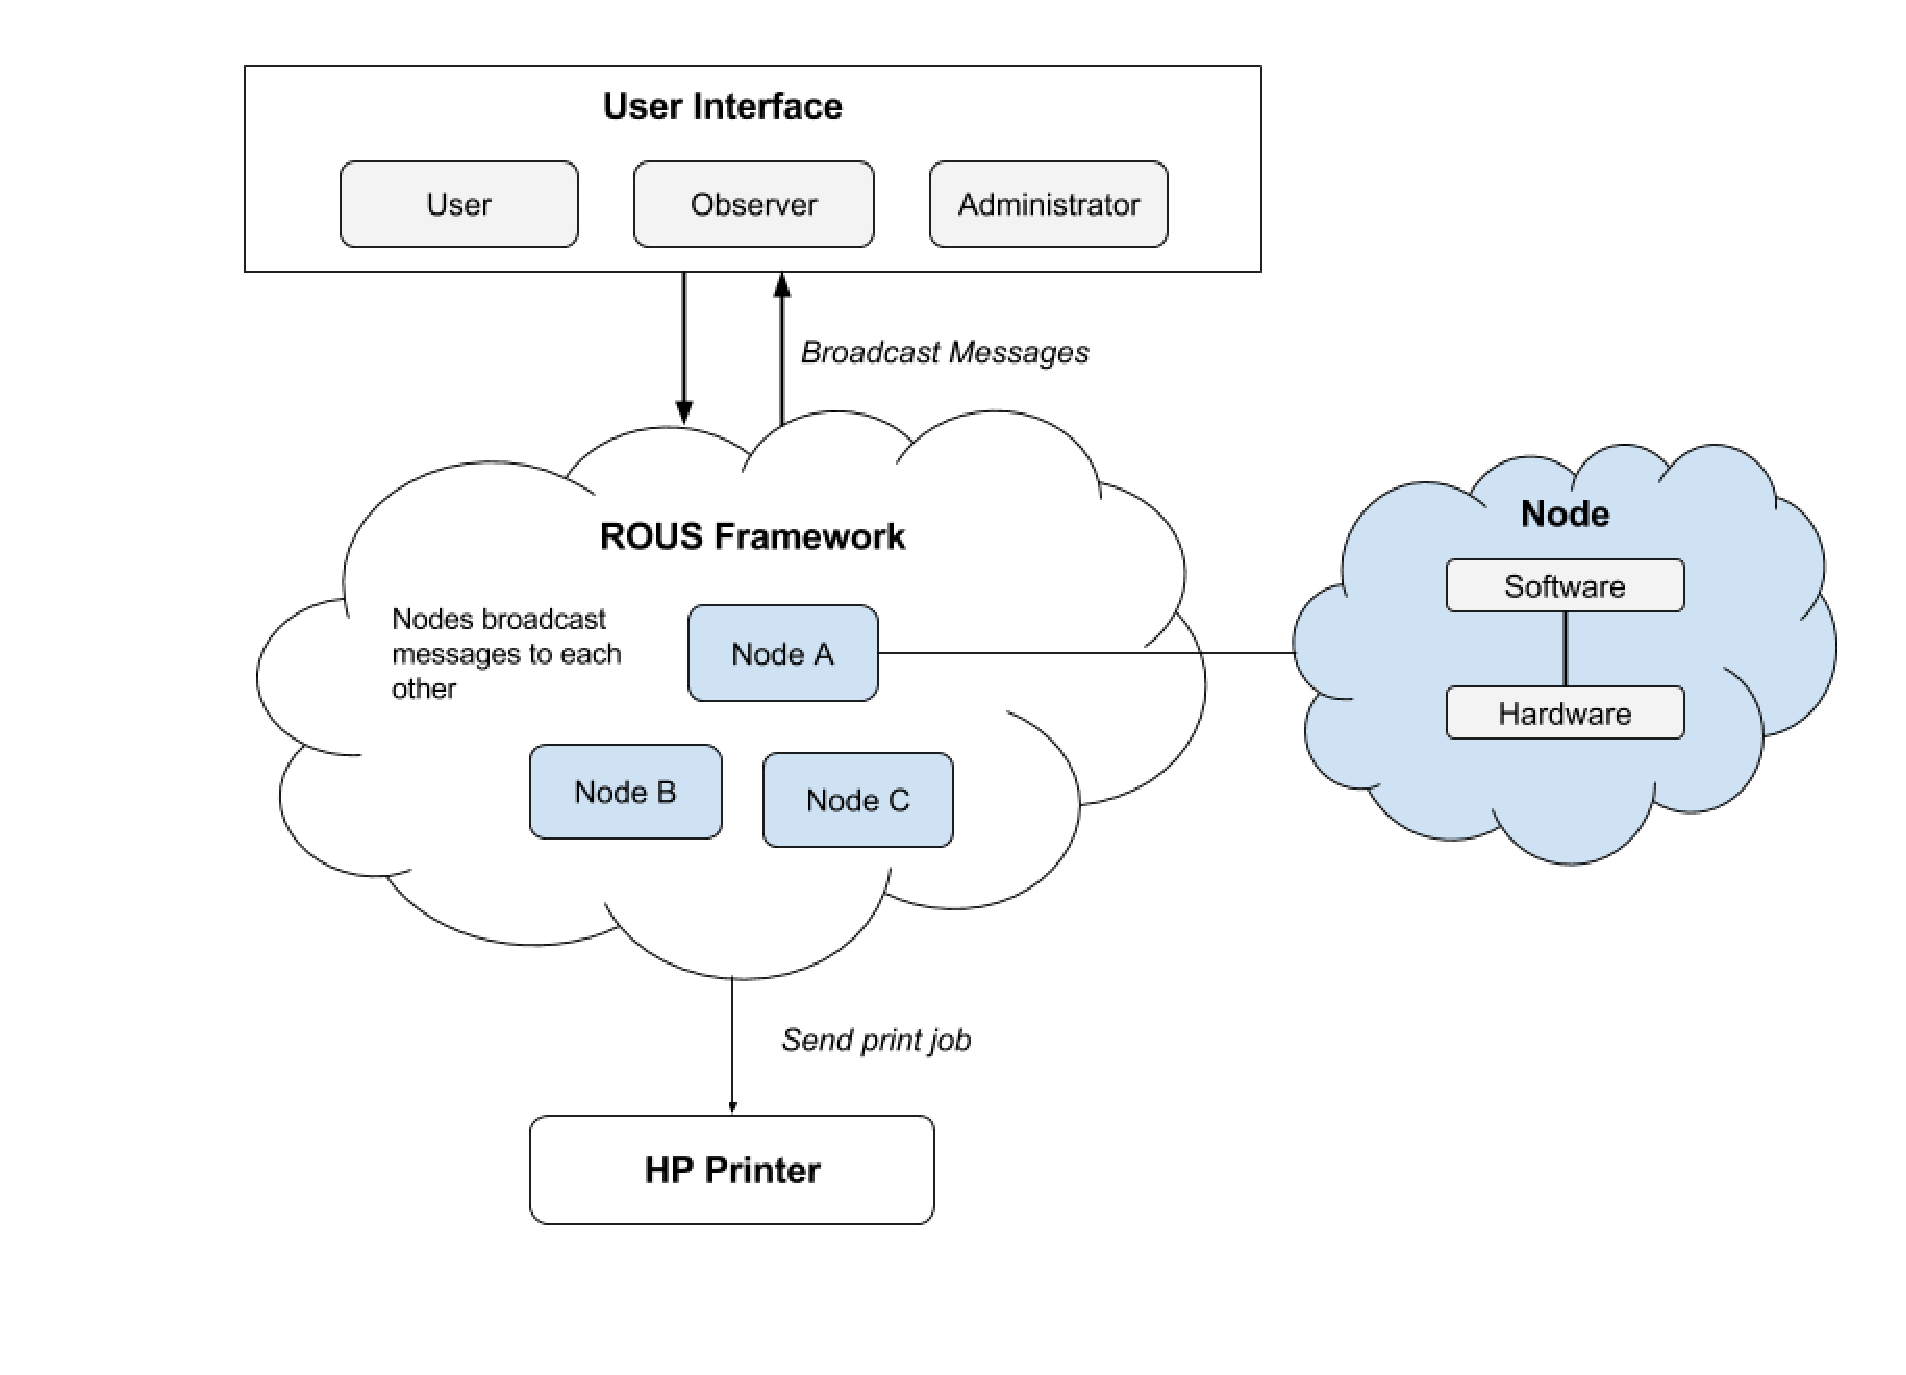
\includegraphics[scale=.45]{context}
	\captionsetup{justification=centering}
    \caption{This is a basic context view of the overall architecture of the ROUS framework}
\end{figure}

\subsection{Goals}
There are a lot of end goals we have for our system. For the system to work as we intend, it shall:
\begin{itemize}
\item Enable nodes to self organize on a structured objective
\item Allow an objective to be input
\item Allow a source of mistrust to be input
\item Output readable configuration data
\item Output readable system state data
\item Output readable results of objective
\item Automatically validate and connect to authorized nodes
\item Allow nodes to share objectives with each other
\item Framework state changes based on the input of a source of mistrust
\item Have a user interface
\item Offer a print service
\end{itemize}


\section{Current Progress}
\subsection{Ongoing Work}
Over winter break and the ten weeks of winter term, most of our time will be spent on the development of our framework. Now that we have a clear view of the requirements and have set how the initial design should look, it is time to start implementation. Using the design document as a starting point, we will begin the process of coding and implementation. 

To start the next step in the project, we will begin by laying out the code structure at a high level. We will write pseudo code and come up with the different pieces that need to be developed. From there we will start implementing the basic pieces of the framework, then work our way up to more complicated functionality. Overall, the next weeks and months will be spent implementing our first alpha level version of our framework.

\subsection{Backlog}
\begin{itemize}
\item Be able to broadcast message
\item Broadcast objective
\item Language keywords
\item Implement language
\item Implement "and" in language
\item Implement "or" in language
\item Task bidding
\item Declare bid winner
\item Task bidding: ties \= rebid
\item Task bidding: ties \= only top tied nodes rebid
\item Carryout objective
\item Node can print to a printer
\item GUI base
\item GUI shows network
\item GUI insert gets file
\item GUI can broadcast to network
\item GUI for administrator
\item GUI for observer
\item GUI for user
\item GUI can receive messages
\end {itemize}



\section{Problems Encountered}
\subsection{Problems}
One of the big problems we had when starting the project was the ambiguity of it all. There was a lot left open for interpretation but this allowed us to create our own project in a sense. Because of this ambiguity, we had to take more time to interpret and create a problem that needed to be solved as well as how we could solve it without needing a doctorate's degree.

Another large issue we faced for most of the term was group dynamics. We had some trouble getting everyone to communicate and contribute to each piece of the project on time and have usable input. Once this escalated we knew very quickly that regular group handling dynamics would not work.

\subsection{Solutions}
To solve the issue of ambiguity, we were able to come up with some time to sit down with our client and talk about our strengths and what we were interested in. The sole requirement of being Internet of Things (IoT) based, we needed to find a problem that needed solving within that scope. After seeing news headlines everywhere over the last couple years and each of us having some interest in the security of both our private networks as well as what the future could hold in terms of security, we settled on a security aspect of IoT frameworks. From this point we came up with the idea of a "mistrusted" node. This is when the collection of nodes can no longer "trust" what one of the nodes is saying or doing and how they work around that to still complete the objective.

After trying techniques that were taught by Ombuds and past life experiences on dealing with differences in a workplace setting, the group dynamic issues were not only persisting, but escalating. We went to our TA, we went to Ombuds, and we finally went to the professors. When things were still escalating further, we went to our college of EECS advisor to get more advice since it was affecting our other classes as well. This problem was resolved by our professors and their solutions have cleared up the issues. 



\section{Retrospective}
\subsection{Overall Summary}
Over the course of fall term our team has made a lot of progress on the project. We have developed a problem statement, finalized the projects requirements, looked at relevant technologies that could be used to implement the project, and finally, discussed in detail how are project is designed. 

We started this term very positive with a lot of motivation for the project. As the first few weeks progressed some group dynamics started to hurt the overall moral of the group. Eventually these issues were resolved. After the issues that plagued the first part of the term were dealt with, the rest of the term went smoothly. Both teammates, Hayden and Kyle, worked together well and communicated to accomplish the papers assigned. We developed a good relationship with our client, Lonnie, and communicate regularly. Our client provides us with excellent feedback which has helped us to improve our work.

Despite the group dynamic issues faced throughout the term, our team was able to overcome persistent issues and work together to have a positive outcome. We worked hard to complete all work assigned and look forward to implementing the framework our the coming weeks and months.


\subsection{Week by Week Summary}
\subsubsection{Week 1}
This week we read and thought about what projects that we wanted to work on. We bid on the projects that we thought were interesting before the assigned deadline. Then throughout the week we researched different ideas related to the projects that we had bid on. We chose what interested me the most as well as some consideration to the companies we would like to work with.  

\subsubsection{Week 2}
This was an exciting week for everyone!

On Tuesday we were assigned to our project and learned who our group members were. Group members meet each other for the first time, exchanged contact information, and discussed their initial impressions of how they saw the project working. Slack was created and each team member shared their individual OneNote with the other members of the team.

Wednesday we contacted our client for the first time. We heard back from Lonnie(client) that same day. Our first client meeting was set up for the next day. We scheduled to have lunch at McMenamins. We also found that we will not have to create any middle-ware onto any existing device but rather use Arduinos or Raspberry Pi's to be the middle man and IoT connectors.

Thursday was our first client meeting. This was a lunch meeting at McMenamins on Monroe. The meeting was productive and a more specific use case for the project was decided on. It was great to meet Lonnie and exciting to get started on this project. We decided to focus on a security portion of Internet of Things and how to mitigate a security break-in with a mesh nodal structure. 

The rest of the week and through the weekend was filled with more discussion among team members on Slack. We discussed and voted on a group name. The group GitHub and blog were created.

\subsubsection{Week 3}
Productive week!

Our team started off the week by finalizing our group project name! 

This week our problem statement rough drafts were due. We were required to bring a copy to class and get advice from fellow students. A project github was created. On Wednesday the group had their first meeting with the assigned TA, Andrew. He outlined what his role is and what he requires from us. We will have weekly meetings with Andrew. Further discussion of the project continues on Slack. 

This week we narrowed down more of what we are going to work on for our project and some specific features we want to focus on. We also met with our TA and set up weekly times for our TA meetings. We also decided to have our weekly review scrum meetings on Tuesdays at 4 with the client, Lonnie. I think we are going to use Raspberry Pi Zero's as nodes.  


\subsubsection{Week 4}
This week we have to finalize our group problem statement and send it to our client by Friday. Our client will need to verify that they received a copy of our problem statement.

On Tuesday we had a productive team meeting. We shared ideas about how we see the project working and what the requirements document might look like. We ran into an issue with Skype and were unable to have a conversion with our client Lonnie. It was a frustrating experience but discovered that it was Skype who was having issues, causing us not to be able to login and having sound issues. Due to these issues Lonnie was kind enough to reschedule for Thursday.
Thursday we had a productive team meeting. Lonnie Skyped in. We discussed our problem statement and how to improve it. We went over different topics related to further narrow down our specific user stories that we will be working towards.  We started discussion on the requirements document.

Friday we got the privilege of getting to go to a lunch meeting on HP campus. Lonnie invited us to a weekly informal lunch meeting where he and his colleagues discuss different topics related to IoT devices and technologies. We were able to introduce our problem to the group and get their insights and feedback. It was enjoyable to listen to people much smarter and more experience on their take on the project. People always have a good way of thinking about project in different lights. After the lunch meeting we got a tour of the HP campus. Very big campus. We got to check out their massive printers and the cool spaces they get to hang out. 

Once we finished the meeting we all grouped up in Lonnie's office to discuss the project. We discussed the development of our user stories. Lonnie made very helpful and insightful comments. He has helped to further focus us on a specific use case and goal. It was a very productive meeting and a really fun afternoon. 

\subsubsection{Week 5}
The goal for this week was to produce a rough draft of the requirements document using the IEEE standard as a guide. On Tuesday we did not have our regular client meeting and had it rescheduled for Thursday. The team meeting on Thursday we had a great feedback from Lonnie on different sections of the requirements document. We were able to get input and hear his thoughts and ideas on how we are moving forward with the requirements document.

This week we finished up  a little more fine tuning on the problem statement and made sure we were all on the same page.  We finished our rough draft of the requirements document, but there is still plenty of editing and adding we need to finish before our final draft. We had a good weekly review meeting on Thursday with Lonnie.I had a talk with Kirsten of some persisting issues and how to handle them. Started to take care of the issues.

\subsubsection{Week 6}
This was a very busy week, we had a meeting with our client, Lonnie, on Monday to talk about some persisting issues and get his advice on how to mitigate that. I also met to get some feedback on our requirements document and sent him a copy of it. All week Hayden and I worked on the requirements document. Lots of work done improving the document, adding images, and reducing the "fluff". We had our weekly TA meeting that Lucien was late to. We also had our weekly review with Lonnie that Lucien did not come to. Tuesday we had a team meeting with the TA and a team Skype meeting with Lonnie. At the Skype meeting Lonnie helped us to remove some of the "design" out of the document. 

Team name and Project name have changed. Project ROUS is the project name with the team name being Rodents of Unusual Size(ROUS). Lots of work all week on the requirements document.

\subsubsection{Week 7}
Finished finalizing the requirements document and getting it approved by Lonnie and approval email sent out to professors.

This was a stressful week when it comes to group dynamic issues. Other than that it was a productive week on our individual technology review document. We have our documents laid out and all technology's picked. We are finishing the research on my last section and finishing up the document before I got back though and correct errors. All and all it was a stressful but productive week.

We finally got Lucien to tell us which part of the project he wanted to write about for the tech review after asking a few times throughout the week. Another main portion is how we are presenting the user with a visual of how the results are being shown. Most of what I am working is the high level directly with user input and output to the user. 


\subsubsection{Week 8}
This week, Kyle and I got to really start focusing on the design portion of the project. We made an appointment with Lonnie to meet on Monday and flesh out a lot of the design for our project and how we are doing it. We decided that creating a threat would be really good to act as if it is an objective for the system. The system will do the objective which would be disabling some service on a node or two. The following objective will have to make it through the system and complete successfully. We also decided on doing a mobile web application using ReactJS so that anyone that is connected to the self-sustained network can connect to the nodes and we may need to create a sign in to have authorized users to see it. The GUI is going to most likely be a Single Page Application (SPA).

Monday we have an in-person client meeting with Lonnie to go over design stuff. Tuesday the rough draft of the tech document was due. We reviewed documents in class and got feedback from another student, this was a graded exercise. Thursday we had meeting with client. We discussed design document and Lonnie gave lots of advice. Wanted us to check out Resin.io.

\subsubsection{Week 9}
This week started out really productive and ended with Thanksgiving, was a good week. Hayden and I had an in person work meeting with Lonnie. Lonnie came to OSU and we had a two hour open discussion about the design of our framework. It was a really productive meeting. He helped answer questions. After the meeting it made it a lot easier for us to dive into the design document. We decided to create a system that bids on services of an objective if the node can do the objective. Each will broadcast a random number and compare their number to the numbers received from broadcasts. If there are no numbers higher than their broadcast number, once the bidding phase is over, it starts the job.

The rest of the week was just spent working on the design doc. Thursday was Thanksgiving and not much work happened on that day. Friday was spent recovering from Thanksgiving. All in all it was a good productive week, and we had a really good meeting with Lonnie.

\subsubsection{Week 10}
Good last week of the term. Had a productive meeting with Lonnie where he gave us really amazing feedback on the Design Document. This feedback helped to improve the document. 

Hayden and I spent the first part of the week finishing up the first draft of the document. On Wednesday we sent the document to Lonnie and he gave us hand written feedback. He gave us some tremendous feedback the following day and we have been working on implementing that since. Then on Thursday during our Skype meeting with Lonnie we got to clarify some questions we had and get more quality feedback from Lonnie.

Friday was sent making changing and cleaning up the different sections that were still not correct. After polishing the document up, I submitted it to GitHub and the OneNote.

\subsection{Reflection Table}
\bgroup
  \def\arraystretch{1.5}
  \resizebox{\textwidth}{!}{
  \begin{tabular}{| p{0.3\linewidth} | p{0.3\linewidth} | p{0.3\linewidth} | }
  \hline	
  \bf{Positives} & \bf{Deltas} & \bf{Actions}\\
  \hline
  Our client, Lonnie, is very helpful and knowledgeable. He has been a great mentor as well as a client. & The backlog needs to have more content & Find more detailed things to implement \\
  \hline
  Lonnie is very engaging & Need more implementation & Allocate more time for development \\
  \hline
  Hayden and Kyle communicate well & Need more pictures/diagrams & Decide which parts need diagrams and create them \\
  \hline
  We got everything turned in on time & Need to define Keyword Language & Come up with some keywords and discuss with each other \\
  \hline
  We received acceptable grades for what we have turned in & ... & ... \\
  \hline
  Professors host a lot of office hours and provide good feedback & ... & ... \\
  \hline
  \end{tabular}
  }
\egroup




\end{document}